\section*{3}

Sean $f_1 , f_2 : \R^n \rightarrow \R$ dos funciones diferenciables y convexas. Se considera la función
\begin{equation*}
    f (x) = \max \{f1 (x), f2 (x)\}.
\end{equation*}
Sea $x_0 \in \R^n$ un punto tal que $f (x_0) = f_1 (x_0) = f_2 (x_0)$.
Pruebe que $l$ es un subgradiente de $f$ en $x_0$ si y sólo si
\begin{equation*}
    l = \lambda \nabla f_1 (x_0) + (1 - \lambda) \nabla f_2 (x_0), \text{ para } \lambda \in [0, 1]. 
\end{equation*}

\noindent\rule{10cm}{0.4pt}

Supongamos que $l$ es de la forma
\begin{equation*}
    l = \lambda \nabla f_1 (x_0) + (1 - \lambda) \nabla f_2 (x_0),
\end{equation*}
con $\lambda \in [0, 1]$.
Entonces
\begin{equation}\label{ex3_ineq}
\begin{aligned}
    f(x_0) + l(x - x_0)
        & = f(x_0) + \lambda \nabla f_1 (x_0) (x - x_0) + (1 - \lambda) \nabla f_2 (x_0) (x - x_0) \\
        & \leq f(x_0) + \lambda (f_1(x) - f_1(x_0)) + (1 - \lambda) (f_2(x) - f_2(x_0)) \\
        & = \lambda f_1(x) + (1 - \lambda) f_2(x) \\
        & \leq f(x),
\end{aligned}
\end{equation}
donde en la primera desigualdad hemos usado el Lema 3.3 del texto base para ver que
\begin{equation*}
    \nabla g (\hat{x}) (x - \hat{x}) \leq g(x) - g(\hat{x}),
\end{equation*}
para toda función $g$ convexa.
Y la desigualdad $(\ref{ex3_ineq})$ confirma que $l \in \partial f(x_0)$.

La idea para ver que todo subgradiente es de la forma
\begin{equation*}
    l = \lambda \nabla f_1 (x_0) + (1 - \lambda) \nabla f_2 (x_0), \text{ para } \lambda \in [0, 1],
\end{equation*}
es porque en el punto $x_0$ dado que las dos funciones coinciden sus dos vectores tangentes se cruzan en $x_0$,
en cada dirección dominara uno u otro en función de si $f_1$ o $f_2$ es mayor que la otra en un pequeño entorno de $x_0$.
Si el subgradiente no esta comprimido entre los dos vectores tangentes entonces en algún punto no se cumplirá la desigualdad $f(x) \geq f(x_0) + l(x - x_0)$.
La Figura \ref{ex3_plot} ilustra esta idea en una dimension.

\begin{figure}[h]
\centering
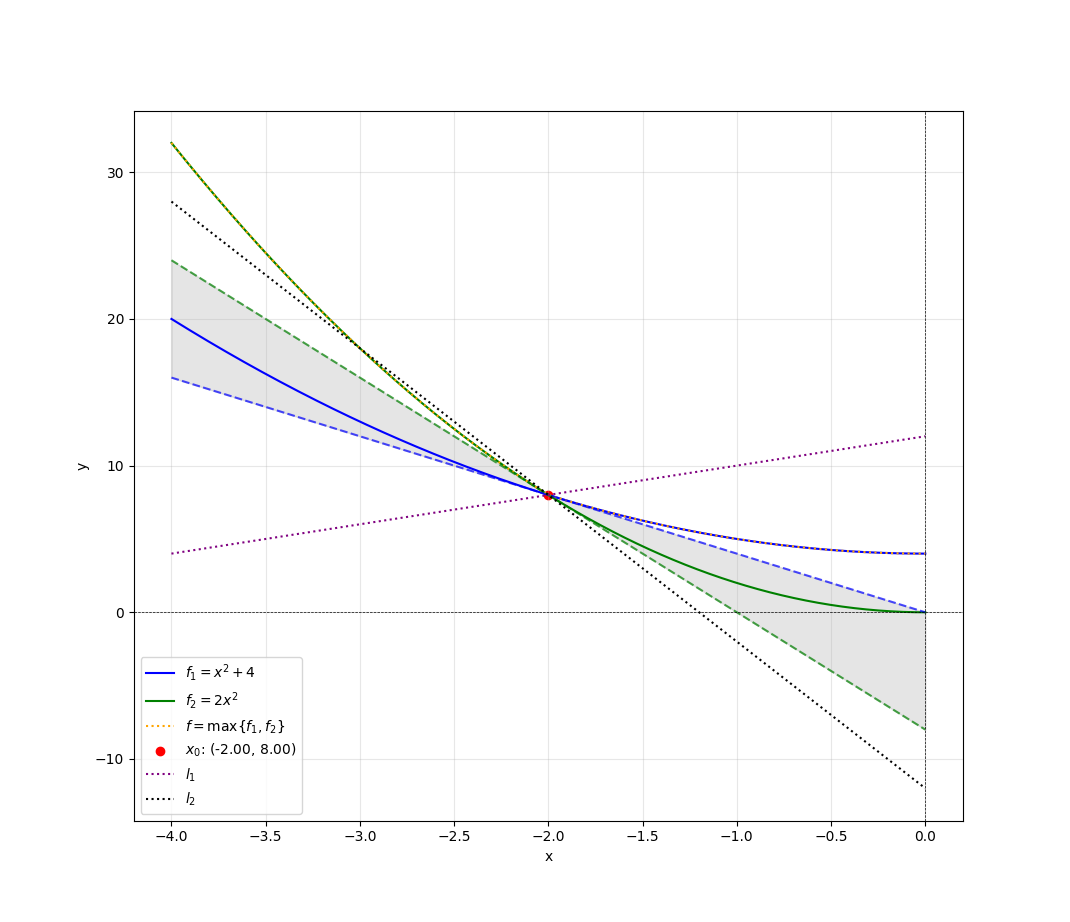
\includegraphics[scale=0.6]{ex3_plot.png}
\caption{
    El gráfico muestra dos funciones convexas y su máximo,
    el area gris es el area comprimida entre los dos vectores tangentes,
    y $l_1, l_2$ son dos vectores que pasan por $x_0$ pero no están en el area gris,
    se ve como no cumplen la desigualdad.
}
\label{ex3_plot}
\end{figure}

Vamos a formalizar la idea.
Sea $l \in \partial f(x_0)$ tal que
\begin{equation*}
    l \neq l_{\lambda} = \lambda \nabla f_1 (x_0) + (1 - \lambda) \nabla f_2 (x_0), \text{ para } \lambda \in [0, 1].
\end{equation*}
Entonces existe $h \in \R^n$ tal que
\begin{equation*}
    l(h) > l_{\lambda}(h), \forall \lambda \in [0, 1] \Rightarrow
    \left\{
    \begin{aligned}
        l(h) > \nabla f_1(x_0)(h), \\
        l(h) > \nabla f_2(x_0)(h). \\
    \end{aligned}
    \right.
\end{equation*}
Sin perdida de generalidad podemos suponer que para un $\alpha > 0$ suficientemente pequeño para que se cumpla
\begin{equation*}
    f(x_0 + \beta h) = f_1(x_0 + \beta h) \geq f_2(x_0 + \beta h), \; \forall 0 \leq \beta \leq \alpha.
\end{equation*}
Y por tanto en la dirección $h$ la derivada direccional de $f$ se corresponde con el gradiente de $f_1$,
\begin{equation*}
    f'(x_0)(h) = \nabla f_1(x_0)(h).
\end{equation*}
Entonces por el Lema 3.25 del texto base tenemos que
\begin{equation*}
    f'(x_0)(h) = \nabla f_1(x_0)(h) \geq l(h) !!
\end{equation*}
que contradice $l(h) > \nabla f_1(x_0)(h)$ y por tanto contradice $l \neq l_{\lambda}$.
Resultando en que $\exists \lambda \in [0,1]$ tal que $l = l_{\lambda}$, como queríamos ver.
